\documentclass{beamer}
\usepackage[utf8]{inputenc}
%\usepackage{minted}
\usepackage{amsmath}
\usepackage{fancyvrb}
\usepackage{xspace}
\usepackage{listings}
%\usepackage{minted}
\usepackage[3D]{movie15}
\usefonttheme{structurebold}
\mode<presentation>
{
  \usetheme{default}
   \setbeamercolor{structure}{fg=black!70}
  %\setbeamercovered{invisible}
  \setbeamerfont{title}{size=\large}
}
\usepackage[english]{babel}
\usepackage{times}
\usepackage[T1]{fontenc}
\usepackage{algorithmic}
%\usepackage[unicode]{hyperref}%$AA 3:55, 720AM 3:40, $748.80 OZAOZF
%how our code can be useful to ERDC in the future
%labwide resource on numerics; and solving problems related to numerical methods and new physical formulations (e.g. femlab)
%maybe add a couple of simulations
\hypersetup{unicode=true,colorlinks=true,linkcolor=black,urlcolor=blue}

%% The Proteus toolkit evolved to support research on new models for
%% coastal and hydraulic processes and improvements in numerical
%% methods. The models considered include multiphase flow in porous
%% media, shallow water flow, turbulent free surface flow, and
%% flow-driven processes such as sediment and species transport. Python
%% was used for implementing high-level class hierarchies and prototyping
%% new algorithms, while performance critical sections were optimized
%% using compiled languages. We discuss the toolkit design,
%% performance, and open issues.
\newcommand{\Jrate}[1]{\stackrel{\circ}{#1}}
\newcommand{\email}[1]{\href{mailto:#1}{\texttt{#1}}}
%differential operators
\newcommand{\grad}{\nabla}
\newcommand{\deld}{\nabla \cdot}
\newcommand{\lap}{\Delta}
%boldface in math mode
\newcommand{\bm}[1]{\mbox{{\boldmath ${#1}$}}}
% vectors and tensors
\renewcommand{\vec}[1]{{\bf #1}}
\newcommand{\gvec}[1]{\mbox{{\boldmath ${#1}$}}}
%mwf comment out bar
%\newcommand{\ten}[1]{\bar{\bm{#1}}}
\newcommand{\ten}[1]{\bm{#1}}
%derivatives
\newcommand{\od}[2]{\frac{d {#1}}{d {#2}}}
\newcommand{\ods}[2]{\frac{d^2{#1}}{d {{#2}^2}}}
\newcommand{\pd}[2]{\frac{\partial {#1}}{\partial {#2}}}
\newcommand{\pds}[2]{\frac{\partial^2{#1}}{\partial {{#2}^2}}}
\newcommand{\pdsm}[3]{\frac{\partial^2{#1}}{\partial {#2}\,\partial {#3}}}
%funtional analysis
\newcommand{\abs}[1]{\left| #1 \right|}
\newcommand{\norm}[1]{\left\| #1 \right\|}
\newcommand{\iprod}[2]{\left( #1, #2 \right)}
\newcommand{\dprod}[2]{\left\langle #1, #2 \right\rangle}
%real numbers
\newcommand{\field}[1]{\mathbb{#1}}
\newcommand{\R}{\field{R}}
\renewcommand{\P}{\field{P}}
\newcommand{\T}{\mathcal{T}}
%funciton spaces
\newcommand{\M}{\mathcal{M}}
%delimiters
\newcommand{\pl}{\left(}
\newcommand{\pr}{\right)}
\newcommand{\sbl}{\left[}
\newcommand{\sbr}{\right]}
\newcommand{\dbl}{\left[\hspace{-0.05cm}\left[}
\newcommand{\dbr}{\right]\hspace{-0.05cm}\right]}
\newcommand{\cbl}{\left\{ }
\newcommand{\cbr}{\right\} }
\newcommand{\eqn}[1]{equation \ref {eq:#1}} 
\newcommand{\Eqn}[1]{Equation \ref {eq:#1}} 
\newcommand{\eqnst}[2]{equations \ref{eq:#1} and \ref{eq:#2}} 
\newcommand{\Eqnst}[2]{Equations \ref{eq:#1} and \ref{eq:#2}} 
\newcommand{\eqns}[2]{equations \ref{eq:#1}--\ref{eq:#2}} 
\newcommand{\Eqns}[2]{Equations \ref{eq:#1}--\ref{eq:#2}}
\newcommand{\msection}[1]{ \vspace{.2in} {\noindent \bf #1}.}
%\renewcommand{\for}{\mbox{for}\quad}
\newcommand{\for}{\mbox{for}\quad}
\newcommand{\argmin}{\mbox{argmin}}
\newcommand{\argmax}{\mbox{argmax}}
\newcommand{\fig}[1]{figure \ref{fig:#1}} 
\newcommand{\Fig}[1]{Figure \ref{fig:#1}} 
\newcommand{\figst}[2]{figures \ref {fig:#1} and \ref {fig:#2}} 
\newcommand{\Figst}[2]{Figures \ref {fig:#1} and \ref {fig:#2}} 
\newcommand{\figs}[2]{figures \ref{fig:#1}--\ref{fig:#2}} 
\newcommand{\Figs}[2]{Figures \ref{fig:#1}--\ref{fig:#2}}
\newcommand{\tab}[1]{table \ref {tab:#1}} 
\newcommand{\Tab}[1]{Table \ref {tab:#1}} 
\newcommand{\tabst}[2]{tables \ref {tab:#1} and \ref {tab:#2}} 
\newcommand{\Tabst}[2]{Tables \ref {tab:#1} and \ref {tab:#2}} 
\newcommand{\tabs}[2]{tables \ref{tab:#1}--\ref{tab:#2}} 
\newcommand{\Tabs}[2]{Tables \ref{tab:#1}--\ref{tab:#2}}
%\newtheorem{theorem}{Theorem}
\newenvironment{neqnarray}[1]{\begin{minipage}[t]{6.5in}  \begin{minipage}[b]{1.0in} #1 \end{minipage}  \begin{minipage}[b]{5.5in}\begin{eqnarray}}{\end{eqnarray}\end{minipage}\end{minipage}}
\newcommand{\bneqnarray}[2]{\\ \\ \fbox{\begin{neqnarray}{#1} #2 \end{neqnarray}}\\ \\ \noindent}

%%%mwf begin adding things
%physical quantities
\newcommand{\source}{b} %or d? or ...
\newcommand{\dx}{\, \mathrm{d}\vec x} 
\newcommand{\ds}{\, \mathrm{d}s}

%finite element quantities
%\newcommand{\Mh}{\mathcal{M}^h}
\newcommand{\Mh}{T_h}
\newcommand{\RT}{$\mbox{RT}_0$}

%\newcommand{\elem}{\mathcal{E}}
%\newcommand{\face}{e}
%\newcommand{\node}{\vec x}
%\newcommand{\nodestar}[1]{\Omega^{#1}}

%element
\newcommand{\elem}{\Omega}
%element boundary (ind. of element)
%\newcommand{\face}{\partial \Omega}
\newcommand{\face}{\gamma}
%mesh nodes
\newcommand{\node}{\vec x}
%node star
\newcommand{\nodestar}[1]{\mathcal{E}({#1})}
%faces in element not on Neumann boundary
\newcommand{\dirIntFaces}[1]{\mathcal{F}_{i}({#1})}
%nodes beloging to an element
\newcommand{\elemnodes}[1]{\mathcal{N}({#1})}
%nodes beloging to an element boundary
\newcommand{\facenodes}[1]{\mathcal{N}({#1})}
%left and right elements at a face
\newcommand{\lelem}{\Omega_{\ell}}
\newcommand{\relem}{\Omega_{r}}
%the left and right identifiers
\newcommand{\eleft}[1]{e_{\ell}({#1})}
\newcommand{\eright}[1]{e_{r}({#1})}
%local numbering on nodestars
\newcommand{\elemstar}{e^{\ast}}
\newcommand{\estarleft}[1]{e^{\ast}_{\ell}({#1})}
\newcommand{\estarright}[1]{e^{\ast}_{r}({#1})}
%left and right normals to face
\newcommand{\lnormal}{\vec{n}_{\ell}}
\newcommand{\rnormal}{\vec{n}_{r}}
%unique normal on face
\newcommand{\fnormal}{\vec{n}_{f}}
%local indeces on left and right
\newcommand{\ileft}{i_{\ell}}
\newcommand{\iright}{i_{r}}
%jump operator
%mwf orig
%\newcommand{\jump}[1]{\dbl #1 \dbr}
%\newcommand{\jump}[2][-0.075cm]{\left[\hspace{#1} \left[ #2 \right]\hspace{#1} \right]}
\newcommand{\jump}[2][\!]{\left[ #1 \left[ #2 \right]#1 \right]}
%multiscale formalism
\newcommand{\strongRes}{\mathcal{R}}
\newcommand{\Lop}{\mathcal{L}}
\newcommand{\LopStar}{\mathcal{L}^{\ast}}
\newcommand{\Ls}{\mathcal{L}_s}
\newcommand{\LsStar}{\mathcal{L}_s^{\ast}}
\newcommand{\LsStarApprox}{\mathcal{L}^{\ast}_{s,h}}
\newcommand{\LsHat}{\hat{\mathcal{L}}_s}
%richards equation stuff
\newcommand{\psk}{$p$-$s$-$k$}

%tables and display convenience
\newcommand{\tx}[1]{$\times 10^{#1}$}
\newcommand{\bit}{\begin{itemize}}
\newcommand{\eit}{\end{itemize}}
\newcommand{\frt}[1]{\frametitle{#1}}

\title[petsc4py]{Multiscale Numerical Modeling of Levee Breach Processes}
%\author[C.~Kees\inst{1} \and M.~Farthing\inst{1}]%
\author[C.~Kees \and M.~Farthing]%
{
  C.~Kees\inst{1}, M.~Farthing\inst{1}, I.~Akkerman\inst{1}\inst{,2}, and Y.~Bazilevs\inst{2}\\ 
  \email{chris.kees@us.army.mil} 
}
\institute[ERDC]
{
 \inst{1}Coastal and Hydraulics Laboratory\\
  US Army Engineer Research and Development Center\\
  Vicksburg, MS, USA\\[10pt]
%\vspace{10pt}
 \inst{2}Department of Structural Engineering\\
  University of Caifornia\\
  San Diego, CA, USA
}
\date [FEMTEC '11]
{
  FEMTEC\\
  May 9 -- 13, 2011
}
\pgfdeclareimage[height=0.5cm]{corps_logo}{corps_logo}
\logo{\pgfuseimage{corps_logo}}

%\AtBeginSection[]
%{
%  \begin{frame}
%    \tableofcontents[currentsection]
%  \end{frame}
%}

%\AtBeginSubsection[]
%{
%  \begin{frame}<beamer>
%    \frametitle{Outline}
%    \tableofcontents[currentsection,currentsubsection]
%  \end{frame}
%}

%\AtBeginSection[]
%{
%  \begin{frame}
%    \tableofcontents[currentsection]
%  \end{frame}
%}

\newcommand{\Cpp}{C\protect\raisebox{.18ex}{++}\xspace}

\begin{document}

\begin{frame}
  \titlepage
\end{frame}

\section*{Outline}

\begin{frame}
\frametitle{Acknowledgments}
\begin{itemize}
\item Lea Jenkins (Clemson University)
\item John Chrispell (Indiana University of Pennsylvania)
\item Tim Kelley (North Carolina State University)
\item Clint Dawson, Steve Mattis, Tim Povich (University of Texas at Austin)
\item Stacy Howington, Jerry Ballard, Maureen Corcoran, John Peters (ERDC)
\end{itemize}
\end{frame}


\begin{frame}
  \frametitle{Outline}
  \begin{itemize}
    \item Overview
    \item Subsurface Processes
    \item Surface Processes
    \item Open Issues
  \end{itemize}
  %\tableofcontents %this is invisible, can't seem to make it visible
\end{frame}

\section{Overview}

\begin{frame}
  \frametitle{Why do we need to simulate Levees?}
  \begin{itemize}
  \item Levees are structures built primarily of earthen materials in order to
    protect large areas from high water.
  \item They typically run along one or both sides of a waterway for very
    large distances and therefore employ cheaper construction
    than dams.
  \item Many are very old and all require continuous maintenance.
  \item We need to model their performance in order to identify
    potential failures and to design new and/or improved levees.
  \end{itemize}
\end{frame}

\begin{frame}
  \frametitle{How do levees function (or fail)?}
    \begin{itemize}
    \item Earthen materials don't hold back water like a
      concrete dam.
    \item The free surface (air/water interface) is continuous as it
      passes from the waterway into the levee.
    \item As water flows through porous media it loses energy to the
      medium through friction, which causes a drop in water pressure.
    \item The result is a free surface that slopes down away from the
      flood side of the levee until it either forms a ``seepage face''
      on the land side of the levee or (preferably) stays under ground.
    \item Failure can result from boils/pipes or from large scale
      stresses arising from pore water pressure and gravity.
    \end{itemize}
\end{frame}

\begin{frame}
\frametitle{2D Seepage Analysis}
\includegraphics[width=4.35in]{sacSteady30.png}
\end{frame}  

\begin{frame}
\frametitle{2D Stability}
\includegraphics[width=2.15in]{wildwood_e.jpg}\includegraphics[width=2.15in]{slopes_e.png}
\end{frame}  

\begin{frame}
\frametitle{2D Stability Analysis}
  \includemovie[controls,poster]{4.25in}{2.5in}{h.mov}
\end{frame}  

\section{Subsurface Processes}

\begin{frame}
  \frametitle{Darcy's law and single phase flow in porous media}
  \begin{itemize}
    \item The water momentum balance in the porous medium takes the
      special form of Darcy's law, which assumes that microscopic
      momentum loss to the soil is linear in the velocity and that
      macroscopic inertial and viscous terms are negligible:
    \begin{equation}
      \grad p - \rho \vec g  + \ten k^{-1} \vec v = 0
    \end{equation}
    \item Combined with fluid mass conservation we usually write the flow equation as
      \begin{equation}
        \deld  -\ten K \grad \phi = 0 
      \end{equation}
      where $\phi = \frac{p}{\rho\|g\|} + z = \psi + z$ is known as the hydraulic head and $\psi$ is known as the pressure head.

  \end{itemize}
\end{frame}

\begin{frame}
  \frametitle{Modeling seepage}
  \begin{itemize}
    \item The seepage problem can be modeled as a free boundary
      problem for single phase flow or as two-phase flow in porous
      media.
    \item In either case boundary conditions along a portion of the
      levee and land surface we have a Signiorini boundary condition:
      \begin{equation}
\psi(\vec v \cdot \vec n) = 0 \quad \vec v \cdot \vec n \geq 0 \quad
\psi \leq 0 \; \vec x \in \Gamma{sf}
      \end{equation}
    \item We will focus on the two-phase approach, more specifically
      Richards' equation, which replaces $K$ with a nonlinear relative
      conductivity $K(\psi)$
      \begin{equation}
        \pd{m(\psi)}{t} + \deld -K(\psi) \grad \phi(\psi) = 0 
      \end{equation}
  \end{itemize}
\end{frame}

\begin{frame}
  \frametitle{Finite element formulation}
  \begin{itemize}
  \item The quantity of interest in seepage modeling is the pressure
    so we use standard Galerkin finite elements on tetrahedra with
    nodal quadrature and element-based material properties.
  \item We use weak enforcement of boundary conditions, for global
    conservation and easier enforcement of the Signiorini condition.
  \item The nonlinear system is solved with Newton's method and a
    simple linear search and various parallel solvers/preconditioners
    from PETSc.
  \end{itemize}
\end{frame}

\begin{frame}
\frametitle{Finite element formulation, ctd.}
\begin{eqnarray}
  (m(\psi_h),w_h)_{L_2(\Omega)} + (K(\psi_h)\grad \phi_h,\grad w_h)_{L_2(\Omega)} + && \\
(-K(\psi_h^-) \grad \phi_h^- \cdot \vec  n + \gamma (\psi_h^- - \psi_h^D),w_h^-)_{L_2(\Gamma^D)} &=& 0
\end{eqnarray}
where $\Gamma^D$ is the actual portion of $\partial \Omega$ with
Dirichlet conditions AND the portion of the Signiorini boundary with
positive with
\begin{equation}
-K(\psi_h^-) \grad \phi_h^- \cdot \vec n + \gamma (\psi_h^-  - \psi_h^D) > 0
\end{equation}
That is, when flow is out of the domain on the Signiorini boundary, enforce $\psi_h^D$
\end{frame}

\begin{frame}
  \includemovie[controls,poster]{4.25in}{2.5in}{phwt2d.mov}
\end{frame}

\begin{frame}
\includegraphics[width=4.35in]{pocketLevee_nopipe.png}
\end{frame}

\begin{frame}
\includegraphics[width=4.35in]{pocketLevee3d_pipe.png}
\end{frame}

\begin{frame}
  \frametitle{Elasto-Plastic Soil Mechanics}
  \begin{itemize}
    \item As with the flow, we model the deformation of the levee by
      treating soil/fluid mixture as a continuum.
      \begin{equation}
        - \deld \ten \sigma  + \vec f = 0
      \end{equation}
      where $\ten \sigma$ is the effective stress tensor, and the pore
      pressure gradient is included in the body forces, $\vec f$, given by
      \begin{equation}
        \vec f = -\rho_s \vec g + \grad p
      \end{equation}
    \item The most significant difficulty is the fact that we have to
      solve a local, nonlinear differential equation involving stress,
      strain, and local ``thermodynamic'' variables (especially near
      slope failures) becomes the soil undergoes {\em plastic}
      strains.
  \end{itemize}
\end{frame}

\begin{frame}
  \frametitle{Stress/Strain rates} A general elastic-plastic material
  response with isotropic hardening given in terms of the Jaumann rate
  of effective stress is
\begin{eqnarray}
\Jrate{\ten{ \sigma}}  &=& \ten D^e (\dot{\ten \epsilon} - \dot{\ten \epsilon}^p) \\
\dot{\ten \epsilon}^p &=& \dot{\lambda} \ten r \\
\dot{q} &=& \dot{\lambda} h \\
\dot{\lambda} &\geq& 0 \\
f(\sigma,q) &\leq& 0
\end{eqnarray}
\end{frame}

\begin{frame}
  \frametitle{Integration of the Stress rate} Writing the rates as
  backward differences and eliminating the time scale since the
  equation is homogeneous gives an algebraic system at each quadrature
  point:
  \begin{eqnarray}
    \Delta \sigma  &=& \ten D^e (\Delta \ten \epsilon - \Delta \ten \epsilon^p) \\
    \Delta \ten \epsilon &=& \Delta \lambda \ten r(\sigma) \\
    \Delta q &=& \Delta \lambda h(\sigma) \\
    \Delta \lambda &\geq& 0 \\
    f(\sigma^{n+1},q^{n+1}) &\leq& 0 
  \end{eqnarray}
where $\ten \sigma = \sigma_n + \Delta \sigma$.
\end{frame}

\begin{frame}
\frametitle{Finite element formulation}
\begin{itemize}
\item Standard linear tetrahedral elements are too ``stiff'' and
  make the structure appear more stable than it is.
\item In this work we use quadratic tetrahedral elements.
\item Structural failure is defined as the point when no stable
  equilibrium solution can be found or when the ratio of plastic
  work to total work becomes large enough.
\item There is typically a spherical failure surface for steep
  slopes.
\end{itemize}
\end{frame}

\begin{frame}
\frametitle{Soil Mechanics Results: Stable Slope}
\includegraphics[width=4.35in]{mcslope.png}
\end{frame}

\begin{frame}
\frametitle{Soil Mechanics Results: Slope Failure}
\includegraphics[width=4.35in]{sgfailure.png}
\end{frame}

\begin{frame}
\frametitle{Coupled Seepage and Stability}
\includegraphics[width=4.35in]{gl_6.png}
\end{frame}

\begin{frame}
\frametitle{LiDAR root scans}
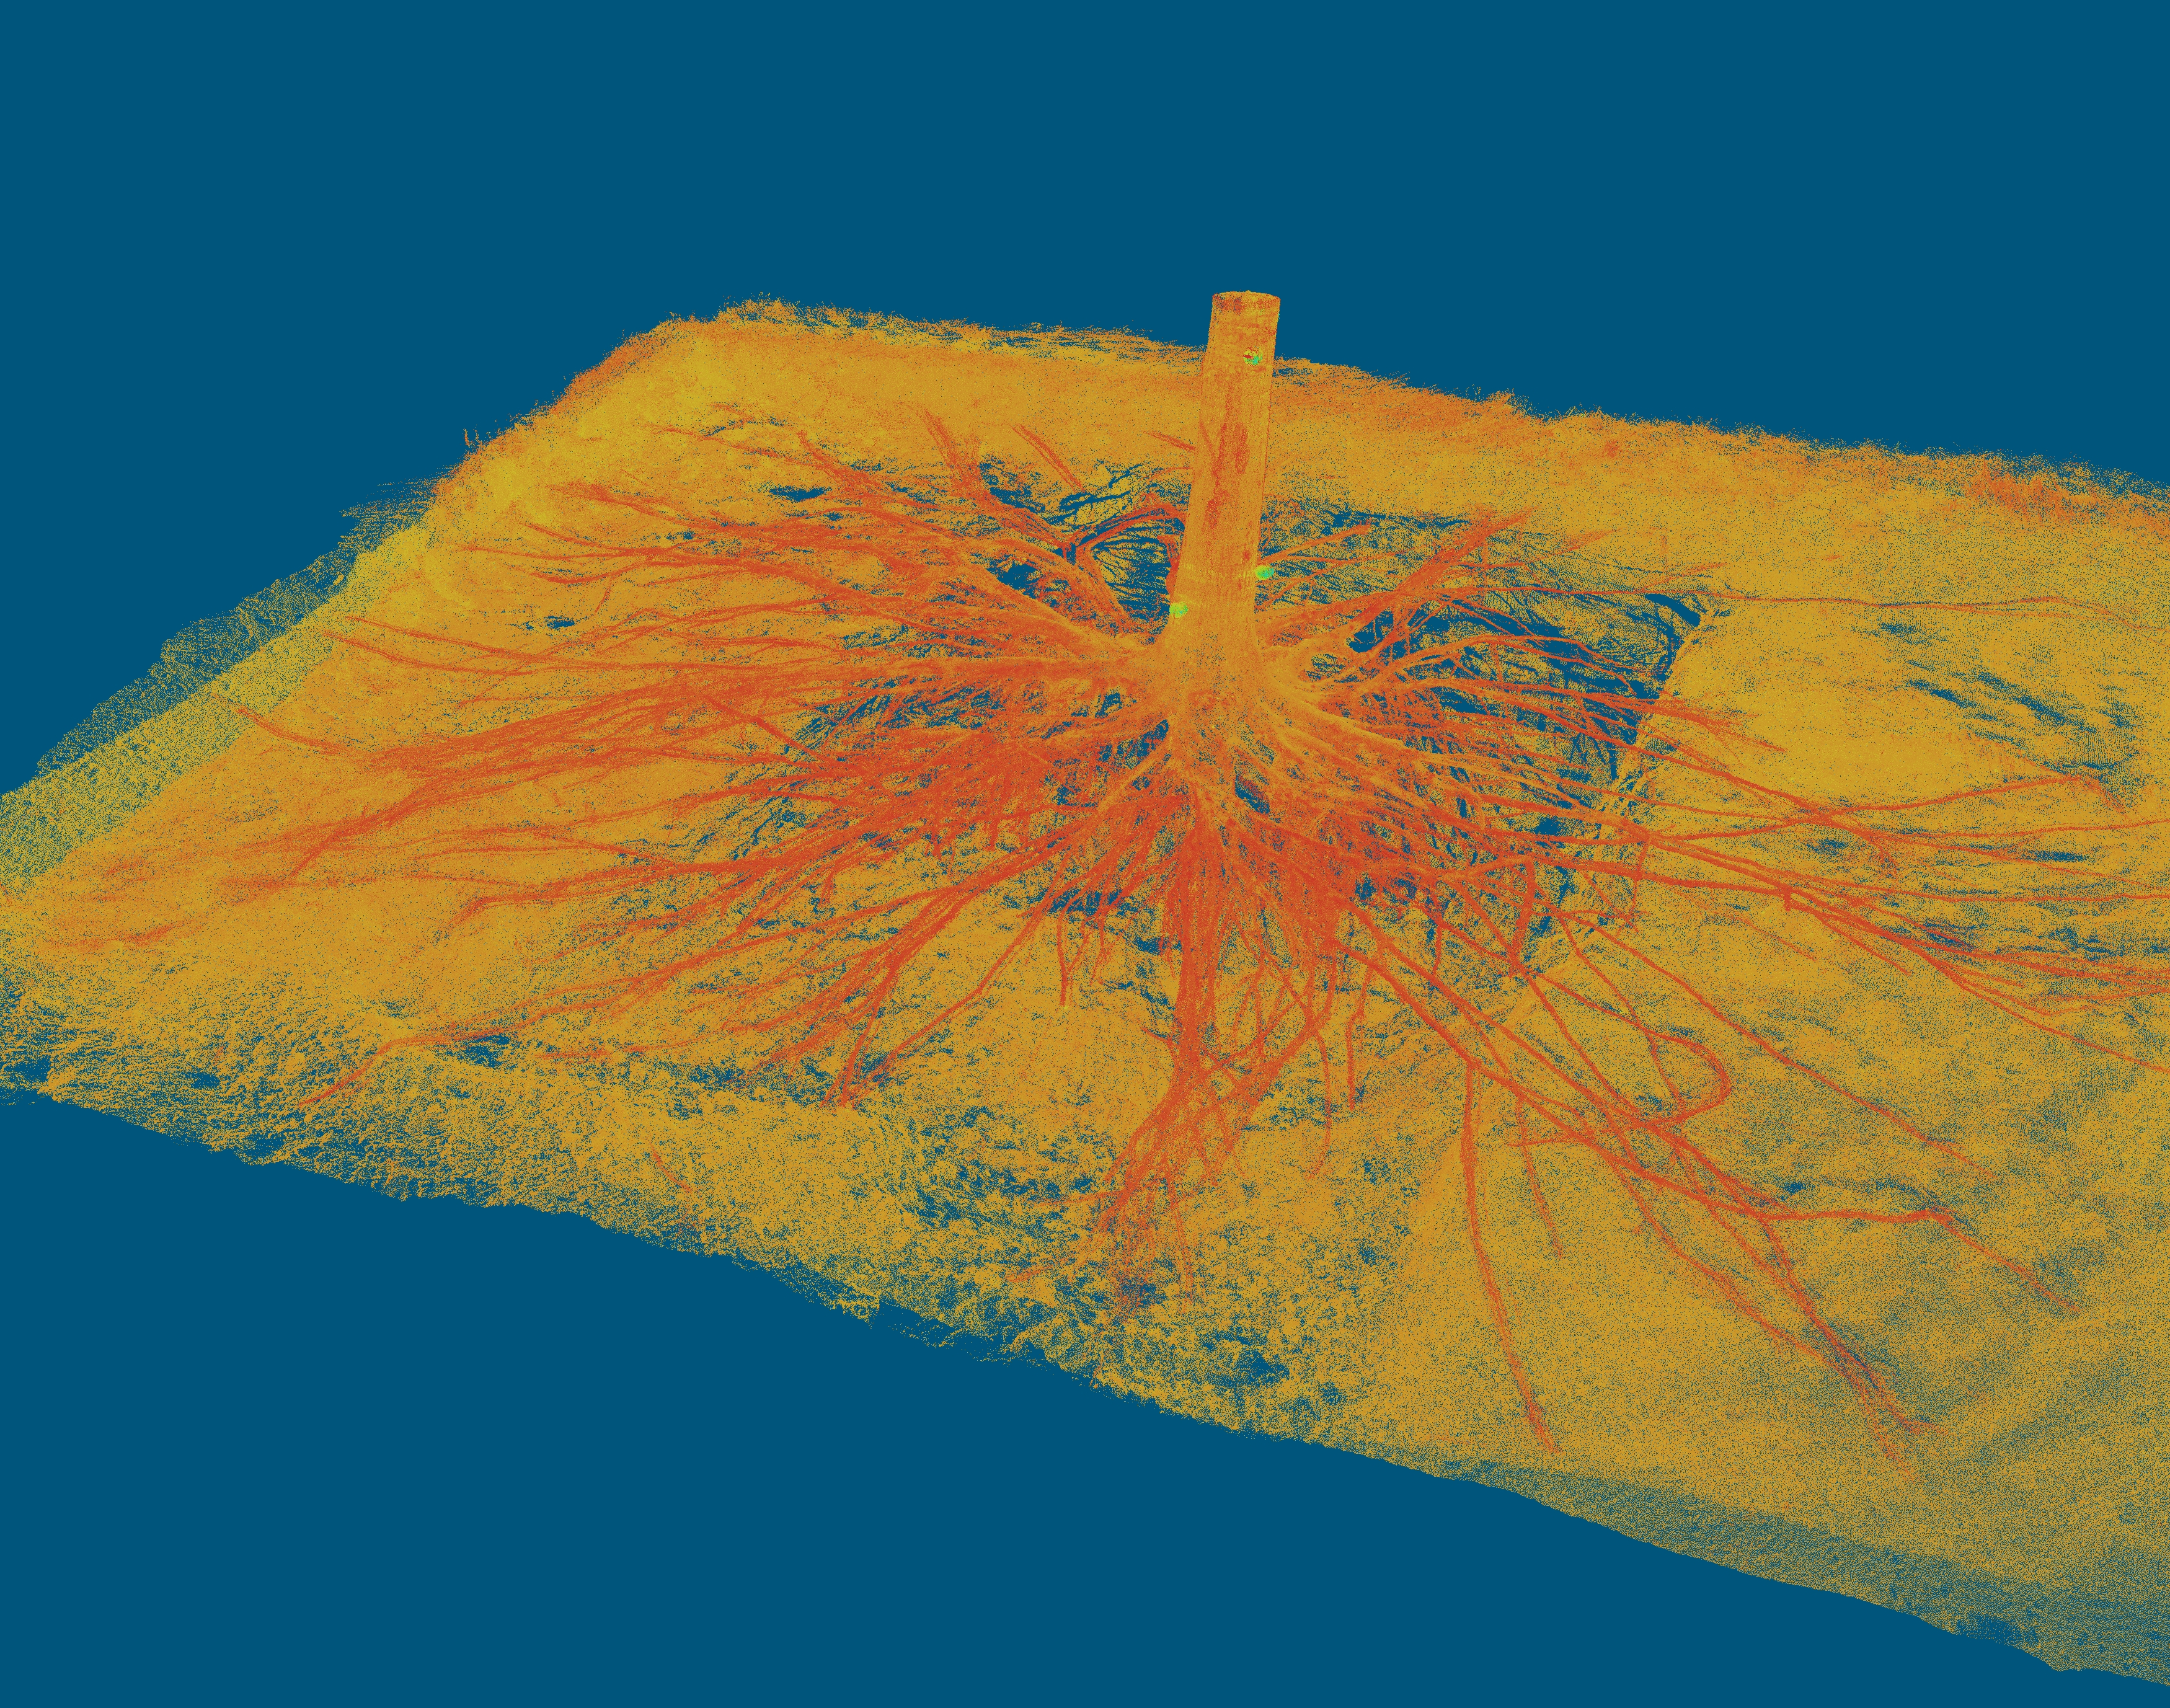
\includegraphics[width=4.35in]{fullRootScan.jpg}
\end{frame}

\begin{frame}
\frametitle{Triangulated surface reconstruction}
\includegraphics[width=4.35in]{rootsPoissonRecon.png}
cite needed for surface recon code
\end{frame}

\begin{frame}
\frametitle{Hand-generated surface reconstruction}
\includegraphics[width=4.35in]{jerry_orig_root_surface.png}
Courtesy Jerry Ballard (cite needed)
\end{frame}

\begin{frame}
\frametitle{Material reclassification approach}
\includegraphics[width=4.35in]{root_zone_coarse_1039766_element_a0_001_tol0_333_block_domain.png}
\end{frame}

\section{Surface Processes}

\begin{frame}{Failure by Overtopping}
\begin{itemize}
\item High-velocity flow forms on land-side slope
\item Shear stress generates rapid erosion 
\item Head cut evolves up slope to generate failure \cite{Briaud_Chen_etal_08}.
\end{itemize}
\end{frame}

\begin{frame}
\frametitle{Process regimes/scales}
\begin{itemize}
\item Sediment-laden mixtures
\item Supercritical and turbulent flow
\item Free surface deformations proportional to depth
\item Fully three-dimensional deformations of free surface and sediment layer (no height function)
\end{itemize}
\end{frame}

\begin{frame}
\frametitle{Existing approaches}
\begin{itemize}
\item Depth-averaged and partly time-averaged (waves)
\item Surface and layer height are unknowns
\item Constitutive relations for morphological processes posed at space/time-integrated scale.
\end{itemize}
\end{frame}

\begin{frame}
\frametitle{St. Venant/Exner System}
\begin{eqnarray}
  \pd{H}{t} + \nabla^{x,y} \cdot \vec U &=& 0\\ %water mass consrv
  \pd{H \vec U}{t} + \nabla^{x,y} \cdot \pl H \vec U \otimes \vec U - \ten{\sigma} \pr  &=& g H \grad{z^{wb}} + S^w \\ %water mom consrv
  \pd{\pl H C \pr}{t} + \nabla^{x,y}\cdot \vec q^s &=& E - D \\ %suspended sed concen
  \pd{\epsilon^s z^{wb}}{t} + \nabla^{x,y} \cdot \pl \vec q^s + \vec q^b \pr &=& - \pd{\pl H C \pr}{t} %moving bed
\end{eqnarray}
\end{frame}

\begin{frame}
\frametitle{Field variables in depth-averaged approach}
\begin{center}
  \def\svgwidth{\textwidth}
  \input{standardModel.pdf_tex}
\end{center}
\end{frame}

\section{Approach}

\begin{frame}
\frametitle{3D Multiphase Approach}
\begin{itemize}
\item Use a fully three-dimensional approach
\item Replace the height function for air/water interface using the level-set approach
\item Replace the bed height function using mixture formulation for sediment/fluid mixture
\item This results in two Navier-Stokes type systems plus some auxiliary equations: $\kappa-\epsilon$(turbulence), $\phi$ (level set)
\item Sediment/fluid coupling formulated in terms of closure relations for fluid/sediment interaction force, $f^{fs}$, stress, and turbulence production.
\end{itemize}
\end{frame}

\begin{frame}
\frametitle{Basic 3D Multiphase Model}
\begin{eqnarray}
  \pd{\rho^f \epsilon^f}{t} + \deld \rho^f \epsilon^f \vec v^f &=& 0 \\ 
  \pd{\rho^f \epsilon^f \vec v^f }{t} + \deld \sbl \rho^f \epsilon^f \vec v^f \otimes \vec v^f - \ten{\sigma^f} \sbr&=& \rho^f \epsilon^f \vec g  - \vec f^{fs} \\
  \pd{\rho^s \epsilon^s}{t} + \deld \rho^s \epsilon^s \vec v^s &=& 0 \\ 
  \pd{\rho^s \epsilon^s \vec v^s}{t} + \deld \sbl \rho^s \epsilon^s \vec v^s \otimes \vec v^s - \ten{\sigma^s} \sbr &=& \rho^s \epsilon^s \vec g  + \vec f^{fs} \\
  \pd{\phi^{aw}}{t} + \epsilon^f \vec v^f \cdot  \grad \phi^{aw} &=& 0 
\end{eqnarray}
\end{frame}

\begin{frame}
\frametitle{Field Variables in 3D Multiphase Model}
\begin{center}
  \def\svgwidth{\textwidth}
  \input{newModel.pdf_tex}
\end{center}
\end{frame}

%% \section{Publication Plan}

%% \begin{frame}
%% \frametitle{Existing Work}
%% \begin{itemize}
%% \item Bakhtyar et. al \cite{Bakhtyar_Barry_etal_09,Bakhtyar_Barry_etal_09b,Bakhtyar_Barry_etal_10} have studied this approach for 2D (cross-shore) beach morphology using a Volume-of-Fluid code.
%% \item Drake and Calantoni described the sediment/fluid interaction force \cite{Drake_Calantoni_01}
%% \item Elghobashi and Abou-Arab described the multiphse turbulence model \cite{Elghobashi_Abou-Arab_83}
%% \end{itemize}
%% \end{frame}

%% \begin{frame}
%% \frametitle{Publication Plan}
%% \begin{itemize}
%% \item ``Three-dimensional numerical simulation of two-phase flow for sediment transport in the inner-surf and swash zones using a hybrid level-set/VOF approach'', Kees, Farthing,...
%% \item Extend Bakhtyar's model to 3D unstructured finite elements, compare to prior 2D work and experiments.
%% \item Add overtopping test problem
%% \end{itemize}
%% \end{frame}
 
\section{Results}

\begin{frame}
\frametitle{Wavetank Test Problem}
\includegraphics[width=\textwidth,keepaspectratio=true]{wavetank.pdf}
\end{frame}

\begin{frame}
\frametitle{Beach Profile Evolution}
\includegraphics[width=\textwidth,keepaspectratio=true]{beachProfile.pdf}
\end{frame}

\begin{frame}
\frametitle{MARIN Experiment}
\includemovie[controls,poster]{\textwidth}{0.75\textheight}{marin500K.mov}
\end{frame}

\begin{frame}
\frametitle{References (Surface)}
\bibliographystyle{plain}
\tiny{\bibliography{femtec2011.bib}}
\end{frame}

\begin{frame}
  \frametitle{References (Subsurface)}
  \begin{footnotesize}
    \begin{itemize}
      
    \item Locally conservative, stabilized finite element methods for
      variably saturated flow. C. E. Kees, M. W. Farthing, and C. N.
      Dawson (2008) {\em Computer Methods in Applied Mechanics and
        Engineering}, 197, 4610-4625.
      
    \item A conservative flux for the continuous Galerkin method based
      on discontinuous enrichment (2004) M. G. Larson and
      A. J. Niklasson. {\em CALCOLO}, 41, 65-76, 2004.
      
    \item Efficient Steady-State Solution Techniques for Variably
      Saturated Groundwater Flow, M. W. Farthing, C. E. Kees,
      T. S. Coffey, C. T. Kelley, and C. T.  Miller (2003) {\em Advances
        in Water Resources}, 26(8), 833-849
      
    \item Versatile Two-level Schwarz Preconditioners for Multiphase Flow,
      C. E. Kees, C. T. Miller, E. W. Jenkins, and C. T. Kelley (2003)
      {\em Computational Geosciences}, 7(2), 91-114
      
    \item Mixed Finite Elements and Higher-Order Temporal Approximations
      for Variably Saturated Groundwater Flow, M. W. Farthing, C. E. Kees,
      and C. T. Miller (2003) {\em Advances in Water Resources}, 26(4),
      373-394
    \end{itemize}
  \end{footnotesize}
\end{frame}

\begin{frame}
  \frametitle{Collaboration, Funding, and Employment Opportunities}
  \begin{itemize}
  \item Partnering and contracting: {\footnotesize
    \url{erdc.usace.army.mil}}
\begin{itemize}
  \item The Broad Area Announcement (BAA) is a standing call for basic
    and applied research proposals
  \item Cooperative Research and Development Agreements (CRADAs) can
    be developed to share staff, equipment, and facilities
\end{itemize}
  \item Post-doctoral positions:\\ {\footnotesize
    \url{www.orau.org/maryland/participants/chl\_projects.html}}
  \item Army Research Office grants in engineering, physics, and
    mathematics:\\ {\footnotesize \url{www.aro.army.mil}}
  \end{itemize}
\begin{center} \large \alert{Thank You!} \end{center}
\end{frame}

\end{document}

% Local Variables:
% mode: latex
% TeX-PDF-mode: t
% End:
